\documentclass[aspectratio=169,10pt]{beamer}

\usetheme{Madrid}
\usecolortheme{seahorse}

\usepackage{amsmath}
\usepackage{amssymb}
\usepackage{amsthm}
\usepackage{xcolor}
\usepackage{listings}
\usepackage{geometry}
\usepackage{graphicx}
\usepackage{hyperref}

\graphicspath{{figures/}}

% Color definitions
\definecolor{darkblue}{rgb}{0, 0, 0.5}
\definecolor{darkgreen}{rgb}{0, 0.5, 0}
\definecolor{darkred}{rgb}{0.5, 0, 0}

% Code listing style
\lstset{
    basicstyle=\ttfamily\scriptsize,
    numbers=left,
    numberstyle=\tiny,
    frame=single,
    breaklines=true,
    columns=fullflexible,
    showstringspaces=false,
    commentstyle=\color{green!50!black}\itshape,
    keywordstyle=\color{blue},
    stringstyle=\color{red},
    language=Python
}

% Beamer settings
\setbeamertemplate{footline}[frame number]
\setbeamerfont{title}{size=\Large}

% Theorem environments
\theoremstyle{definition}
\newtheorem{proposition}{Proposition}
\newtheorem{corollary}{Corollary}
\newtheorem{remark}{Remark}

\title{Chapter 18: Further Differentiability Results}
\subtitle{Calculus of Subdifferentials in Convex Analysis}
\author{Based on Bauschke \& Combettes (2017)}
\date{2024}

\begin{document}

% ============================================================================
% TITLE SLIDE
% ============================================================================

\begin{frame}
  \titlepage
\end{frame}

% ============================================================================
% OUTLINE
% ============================================================================

\begin{frame}{Chapter Overview}
\tableofcontents
\end{frame}

% ============================================================================
% SECTION 1: EKELAND-LEBOURN THEOREM
% ============================================================================

\section{18.1 The Ekeland-Lebourn Theorem}

\begin{frame}[allowframebreaks]{The Ekeland-Lebourn Theorem}

\textbf{Key Idea:} For a convex function that is continuous at a point, Fréchet
differentiability holds on a \emph{dense} $G_\delta$ subset of the domain.

\vspace{0.3cm}

\begin{theorem}[Ekeland-Lebourn]
Let $f: \mathcal{H} \to [-\infty, +\infty]$ be convex, and suppose that
$\text{cont } f \neq \emptyset$. Then the set of points at which $f$ is
\textbf{Fréchet differentiable} is a dense $G_\delta$ subset of $\text{dom } f$.
\end{theorem}

\vspace{0.3cm}

\textbf{Explanation:}
\begin{itemize}
  \item A $G_\delta$ set is a countable intersection of open sets
  \item ``Dense'' means the closure equals the whole space
  \item This is a powerful result: while $f$ may not be differentiable everywhere,
        it is differentiable ``almost everywhere'' in a topological sense
  \item The proof uses:
    \begin{itemize}
      \item Proposition 18.2 (the set $S_\varepsilon$ from the text)
      \item Continuity properties of convex functions (Theorem 8.38)
      \item Local boundedness of $f$
    \end{itemize}
\end{itemize}

\vspace{0.3cm}

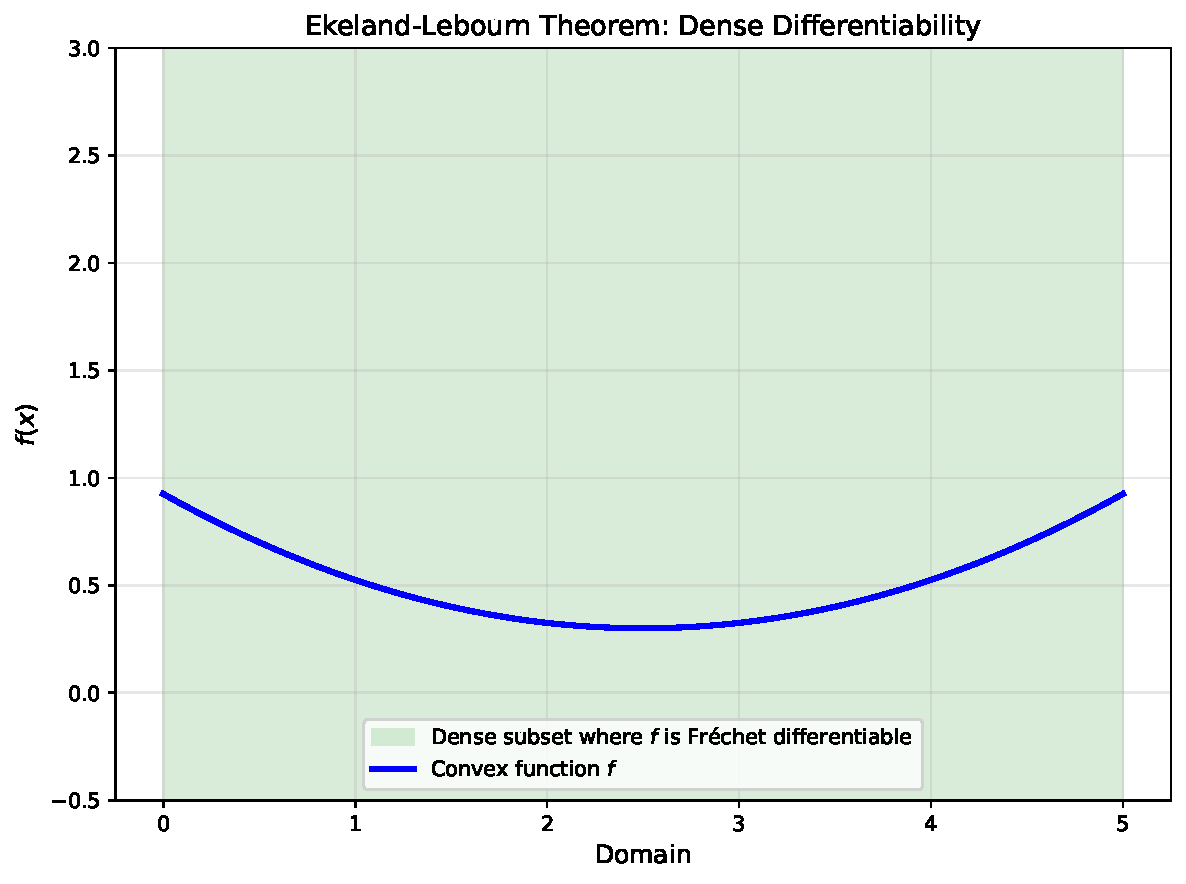
\includegraphics[width=0.6\textwidth]{fig_ekeland_lebourn.pdf}

\end{frame}

\begin{frame}{Ekeland-Lebourn: Key Insights}

\textbf{Proof Strategy:}

\begin{enumerate}
  \item For $\varepsilon > 0$, define the set:
  $$S_\varepsilon = \bigcup_{\eta \in \mathbb{R}_{++}} \left\{ x \in \text{cont } f \, \bigg| \,
    \sup_{y \in H, \|y\|=1} \frac{f(x+\eta y) + f(x-\eta y) - 2f(x)}{\eta} < \varepsilon \right\}$$

  \item This set is \textbf{open} and \textbf{dense} by Proposition 18.2

  \item The intersection $S = \bigcap_{n \in \mathbb{N} \setminus \{0\}} S_{1/n}$
        is a dense $G_\delta$ set

  \item On $S$, the function $f$ satisfies the Fréchet differentiability condition
\end{enumerate}

\vspace{0.3cm}

\textbf{Intuition:} The oscillations of $f$ become arbitrarily small when restricted
to a small enough neighborhood, which forces Fréchet differentiability.

\vspace{0.3cm}

\textbf{Significance for Convex Analysis:}
\begin{itemize}
  \item Shows that convexity + continuity $\Rightarrow$ ``almost everywhere'' smoothness
  \item Motivates the study of subdifferentials (more general than gradients)
  \item Foundation for optimization algorithms that require differentiability
\end{itemize}

\end{frame}

% ============================================================================
% SECTION 2: SUBDIFFERENTIAL OF MAXIMUM
% ============================================================================

\section{18.2 The Subdifferential of a Maximum}

\begin{frame}[allowframebreaks]{Subdifferential of a Maximum Function}

\textbf{Problem:} How do subdifferentials behave when we take the pointwise maximum
of multiple convex functions?

\vspace{0.3cm}

\begin{theorem}[Dubovitskii and Milyutin]
Let $(f_i)_{i \in I}$ be a finite family of convex functions from $\mathcal{H}$ to
$[-\infty, +\infty]$, and suppose that
$x \in \bigcap_{i \in I} \text{cont } f_i$.

Define $f = \max_{i \in I} f_i$ and $I(x) = \{i \in I \mid f_i(x) = f(x)\}$.

Then:
$$\partial f(x) = \text{conv } \bigcup_{i \in I(x)} \partial f_i(x).$$
\end{theorem}

\vspace{0.3cm}

\textbf{Key Points:}
\begin{itemize}
  \item $I(x)$ is the set of indices where the maximum is achieved
  \item The subdifferential of the max is the convex hull of the union of
        subdifferentials at active functions
  \item This is the \emph{subdifferential calculus rule for maximum}
\end{itemize}

\vspace{0.3cm}

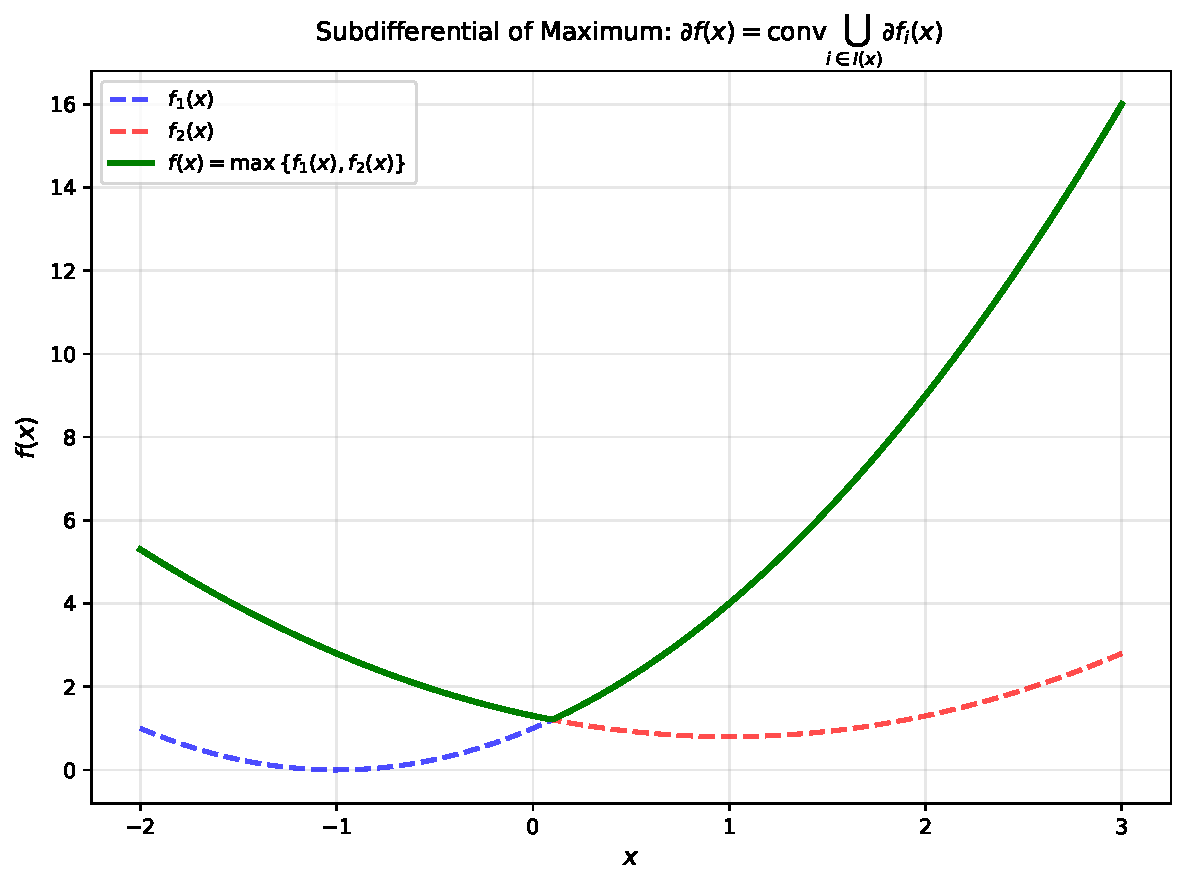
\includegraphics[width=0.7\textwidth]{fig_subdifferential_max.pdf}

\end{frame}

\begin{frame}{Dubovitskii-Milyutin: Proof Outline}

\textbf{Proof uses contradiction:}

\begin{enumerate}
  \item Assume strict inclusion: $\partial f(x) \setminus \text{conv} \bigcup_{i \in I(x)} \partial f_i(x) \neq \emptyset$

  \item Let $u$ be in this difference. By Theorem 3.50 (separation theorem), there exist
        $y \in \mathcal{H} \setminus \{0\}$ and $\varepsilon > 0$ such that:
        $$\langle y | u \rangle \geq \varepsilon + \max_{i \in I(x)} \sup \langle y | \partial f_i(x) \rangle$$

  \item For $u \in \partial f(x)$, convexity gives:
        $$\langle y | u \rangle \geq \max_{i \in I(x)} f_i'(x; y) = f'(x; y)$$

  \item But $u \notin \text{conv} \bigcup_{i \in I(x)} \partial f_i(x)$ leads to a contradiction
\end{enumerate}

\vspace{0.3cm}

\textbf{Result:} The subdifferential is completely determined by the active functions.

\end{frame}

% ============================================================================
% SECTION 3: INFIMAL CONVOLUTIONS
% ============================================================================

\section{18.3 Differentiability of Infimal Convolutions}

\begin{frame}[allowframebreaks]{Infimal Convolutions: Overview}

\textbf{Definition:} The \emph{infimal convolution} of $f, g \in \Gamma_0(\mathcal{H})$ is:
$$f \square g(x) = \inf_{y \in \mathcal{H}} \{f(y) + g(x - y)\}$$

\vspace{0.3cm}

\begin{proposition}[Differentiability of Infimal Convolution]
Let $f, g \in \Gamma_0(\mathcal{H})$, and let $x, y \in \mathcal{H}$.

Suppose that $x \in \text{dom} \partial (f \square g)$,
$f \square g(x) = f(y) + g(x-y)$, and $f$ is Gâteaux differentiable at $y$.

Then:
$$\partial(f \square g)(x) = \{\nabla f(y)\}.$$
\end{proposition}

\vspace{0.3cm}

\textbf{Key Insight:}
\begin{itemize}
  \item The infimal convolution simplifies the subdifferential
  \item When $f$ is differentiable at the minimizer $y$, the subdifferential becomes a singleton
  \item This is crucial for variational analysis and optimization
\end{itemize}

\vspace{0.3cm}

\begin{corollary}
If $f$ is real-valued, supercoercive, and Fréchet differentiable on $\mathcal{H}$,
then $f \square g$ is Fréchet differentiable on $\mathcal{H}$ with:
$$\nabla(f \square g) = \nabla f.$$
\end{corollary}

\end{frame}

% ============================================================================
% SECTION 4: DIFFERENTIABILITY AND STRICT CONVEXITY
% ============================================================================

\section{18.4 Differentiability and Strict Convexity}

\begin{frame}{Strict Convexity and Differentiability: Duality}

\textbf{Central Question:} What is the relationship between differentiability of
$f$ and strict convexity of $f^*$?

\vspace{0.3cm}

\begin{proposition}[Differentiability implies strict convexity of dual]
Let $f \in \Gamma_0(\mathcal{H})$ be such that $f^*$ is strictly convex on every
nonempty convex subset of $\text{dom} \partial f^*$.

Then $f$ is Gâteaux differentiable on $\text{int dom } f$.
\end{proposition}

\vspace{0.3cm}

\begin{proposition}[Strict convexity implies differentiability of dual]
Let $f \in \Gamma_0(\mathcal{H})$ be Gâteaux differentiable on $\text{int dom } f$.

Then $f^*$ is strictly convex on every nonempty convex subset of $\nabla f(\text{int dom } f)$.
\end{proposition}

\vspace{0.3cm}

\begin{corollary}[Complete Characterization]
Suppose $\text{dom } \partial f = \text{int dom } f$ and $\text{dom } \partial f^* = \text{int dom } f^*$.

Then $f$ is Gâteaux differentiable on $\text{int dom } f$ if and only if $f^*$ is
strictly convex on $\text{int dom } f^*$.
\end{corollary}

\vspace{0.2cm}

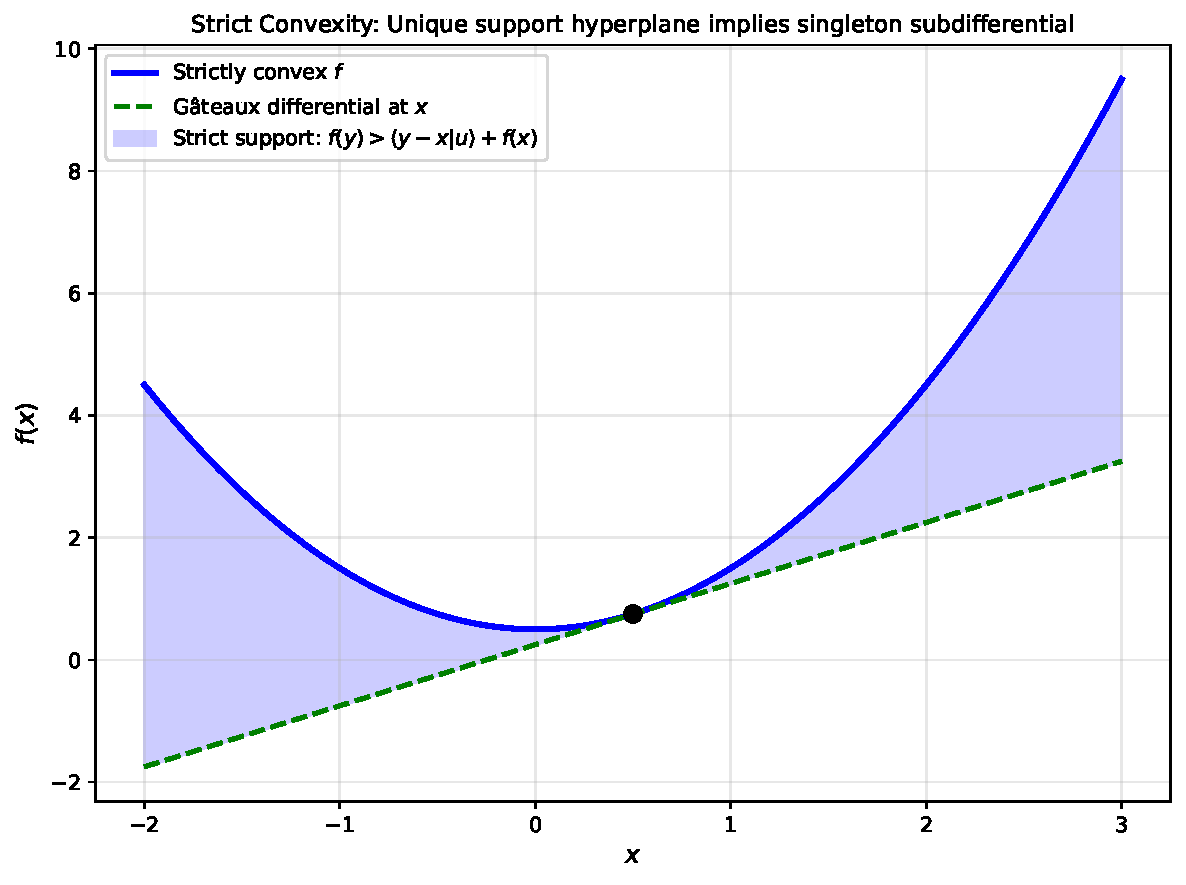
\includegraphics[width=0.6\textwidth]{fig_strict_convexity.pdf}

\end{frame}

% ============================================================================
% SECTION 5: STRONGER NOTIONS OF DIFFERENTIABILITY
% ============================================================================

\section{18.5 Stronger Notions of Differentiability}

\begin{frame}[allowframebreaks]{Stronger Differentiability Concepts}

\textbf{Beyond Fréchet differentiability:} We study gradient continuity and uniform growth.

\vspace{0.3cm}

\begin{theorem}[Characterization of Lipschitz Continuous Gradients]
Let $f: \mathcal{H} \to \mathbb{R}$ be Fréchet differentiable, and let $\phi: \mathbb{R} \to \mathbb{R}_+$
be an even convex function that vanishes only at $0$.

Define $\psi(s) = \frac{\phi(s)}{|s|}$ for $s \neq 0$, $\psi(0) = 0$, and $\theta(s) = \int_0^1 \frac{\phi(st)}{t} dt$.

Then all of the following are equivalent:
\begin{enumerate}
  \item[(i)] $(\forall x, y \in \mathcal{H})(\|\nabla f(x) - \nabla f(y)\| \leq \psi(\|x - y\|))$

  \item[(ii)] $(\forall x, y \in \mathcal{H})(\langle x - y | \nabla f(x) - \nabla f(y) \rangle \leq \phi(\|x - y\|))$

  \item[(iii)] $(\forall x, y \in \mathcal{H})(f(y) \leq f(x) + \langle y - x | \nabla f(x) \rangle + \theta(\|x - y\|))$
\end{enumerate}

And (i)$\Rightarrow$(ii)$\Rightarrow$(iii)$\Rightarrow$(iv)$\Rightarrow$(v)$\Rightarrow$(vi).
\end{theorem}

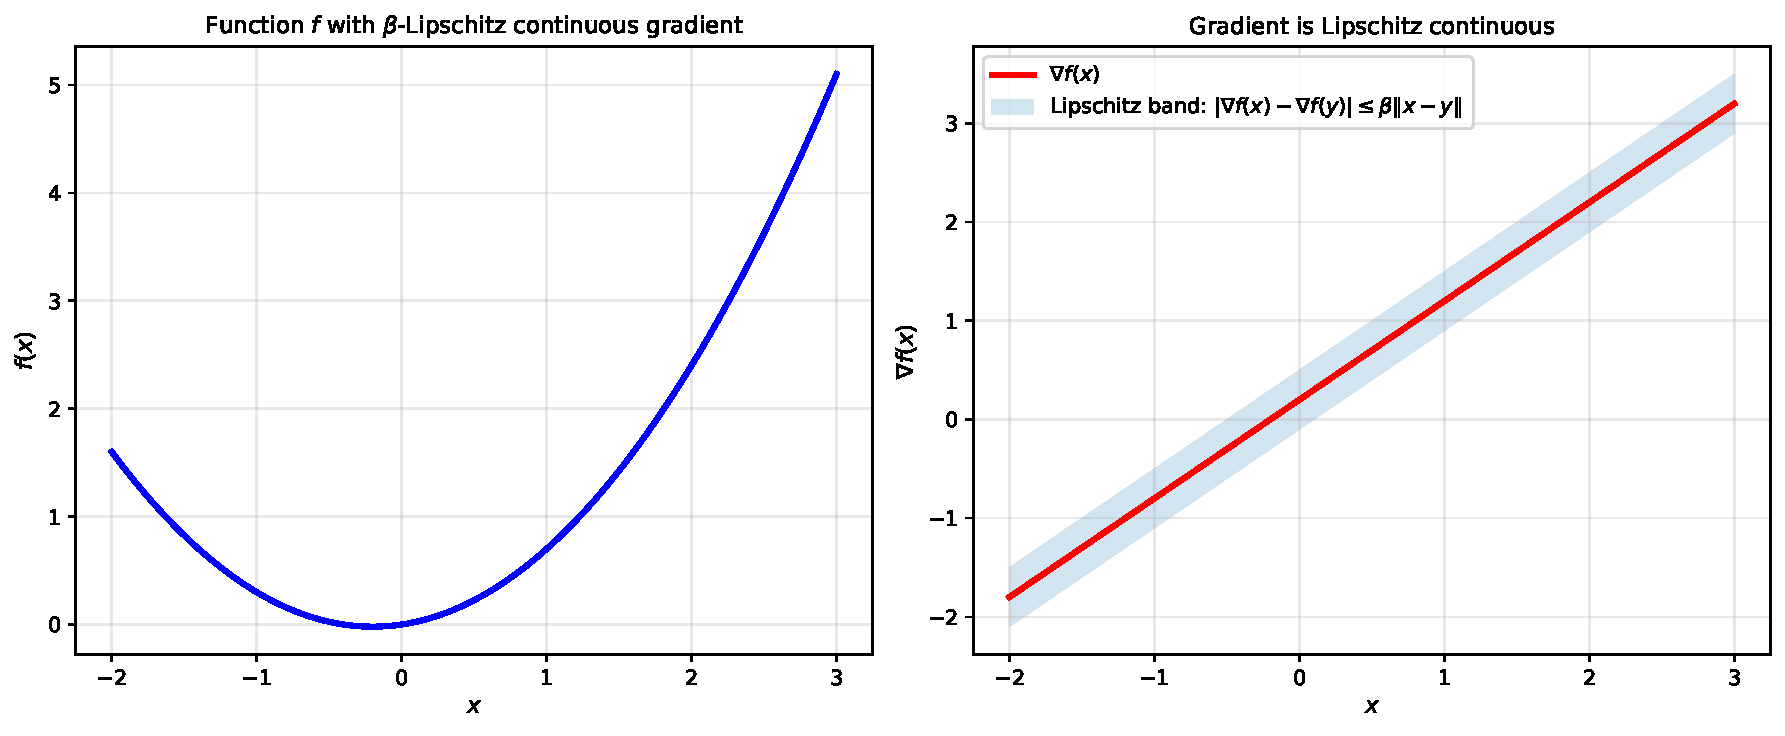
\includegraphics[width=0.7\textwidth]{fig_lipschitz_gradient.pdf}

\end{frame}

\begin{frame}{Lipschitz Continuous Gradients: Important Cases}

\textbf{Special Case: Hölder Continuous Gradients}

\begin{corollary}[Hölder Continuous Gradients]
Let $f: \mathcal{H} \to \mathbb{R}$ be Fréchet differentiable, $\beta \in \mathbb{R}_{++}$,
and $p \in [0,1]$. Consider the following statements:

\begin{enumerate}
  \item[(i)] $(\forall x, y \in \mathcal{H})(\|\nabla f(x) - \nabla f(y)\| \leq \beta\|x - y\|^p)$

  \item[(ii)] $(\forall x, y \in \mathcal{H})(\langle x - y | \nabla f(x) - \nabla f(y) \rangle \leq \beta\|x - y\|^{p+1})$

  \item[(iii)] $(\forall x, y \in \mathcal{H})(f(y) \leq f(x) + \langle y - x | \nabla f(x) \rangle + \beta(p+1)^{-1}\|x - y\|^{p+1})$
\end{enumerate}

Then (i)$\Rightarrow$(ii)$\Rightarrow$(iii)$\Rightarrow$(iv)$\Rightarrow$(v)$\Rightarrow$(vi).
\end{corollary}

\vspace{0.3cm}

\textbf{Most Important Special Case: $\beta$-Smooth Functions}

When $p = 1$, we get the classical notion of $\beta$-Lipschitz continuous gradients:
$$\|\nabla f(x) - \nabla f(y)\| \leq \beta\|x - y\|$$

This is also called \emph{$\beta$-smoothness} or the gradient being $\beta$-Lipschitz continuous.

\end{frame}

\begin{frame}{Baillon-Haddad Theorem}

\begin{corollary}[Baillon-Haddad]
Let $f: \mathcal{H} \to \mathbb{R}$ be a Fréchet differentiable convex function and
$\beta \in \mathbb{R}_{++}$.

Then $\nabla f$ is $\beta$-Lipschitz continuous if and only if $\nabla f$ is
$(1/\beta)$-cocoercive.

In particular, $\nabla f$ is nonexpansive if and only if $\nabla f$ is firmly nonexpansive.
\end{corollary}

\vspace{0.3cm}

\textbf{Cocoercivity Definition:}
An operator $A$ is $\alpha$-cocoercive if:
$$\langle x - y | Ax - Ay \rangle \geq \alpha \|Ax - Ay\|^2$$

\vspace{0.3cm}

\textbf{Significance:}
\begin{itemize}
  \item Links differentiability properties with operator monotonicity
  \item $(1/\beta)$-cocoercivity is weaker than $\beta$-Lipschitz continuity
  \item Crucial for monotone operator theory and fixed point algorithms
\end{itemize}

\end{frame}

\begin{frame}{Moreau Envelope and Regularization}

\begin{corollary}[Moreau Envelope]
Let $f \in \Gamma_0(\mathcal{H})$, $\beta \in \mathbb{R}_{++}$, and
$q = (1/2)\|\cdot\|^2$. Then $f$ is Fréchet differentiable on $\mathcal{H}$
with a $\beta$-Lipschitz continuous gradient if and only if $f$ is the
Moreau envelope of parameter $1/\beta$ of a function in $\Gamma_0(\mathcal{H})$:
$$f = \left(f^* - \frac{1}{\beta}q\right)^* \square \beta q.$$
\end{corollary}

\vspace{0.3cm}

\textbf{Moreau Envelope:}
$$m_\gamma(f)(x) := \inf_y \left\{ f(y) + \frac{1}{2\gamma}\|x - y\|^2 \right\}$$

\vspace{0.3cm}


\includegraphics[width=0.6\textwidth]{fig_moreau_envelope.pdf}

\vspace{0.2cm}

\textbf{Properties:}
\begin{itemize}
  \item Always smooth (differentiable) if the original function $f$ is proper and convex
  \item Gradient is Lipschitz continuous with constant $1/\gamma$
  \item Foundation for proximal gradient methods
\end{itemize}

\end{frame}

\begin{frame}{Proximal Operators and Averaged Proximal Operators}

\begin{corollary}[Averaged Proximal Operators]
Let $(f_i)_{i \in I}$ be a finite family of functions in $\Gamma_0(\mathcal{H})$,
let $(\alpha_i)_{i \in I}$ be a finite family of real numbers in $[0,1]$ such that
$\sum_{i \in I} \alpha_i = 1$, and set $q = (1/2)\|\cdot\|^2$.

Then $\sum_{i \in I} \alpha_i \text{Prox}_{f_i}$ is the proximity operator of a
function $h \in \Gamma_0(\mathcal{H})$:
$$\sum_{i \in I} \alpha_i \text{Prox}_{f_i} = \text{Prox}_h, \quad
\text{where } h = \left( \sum_{i \in I} \alpha_i (f_i^* \square q) \right)^* - q.$$
\end{corollary}

\vspace{0.3cm}

\textbf{Key Application:}
\begin{itemize}
  \item Shows how to average proximal operators
  \item Important for parallel optimization algorithms
  \item Special case: $\alpha_1 = \alpha_2 = 1/2$ gives the proximal average
\end{itemize}

\end{frame}

% ============================================================================
% SECTION 6: DISTANCE TO A SET
% ============================================================================

\section{18.6 Differentiability of the Distance to a Set}

\begin{frame}[allowframebreaks]{Distance Function to a Convex Set}

\textbf{Definition:} For a nonempty closed convex set $C \subseteq \mathcal{H}$:
$$d_C(x) = \inf_{z \in C} \|x - z\|$$

\textbf{Question:} When is $d_C$ differentiable, and what is its subdifferential?

\vspace{0.3cm}

\begin{proposition}[Differentiability Characterization]
Let $C$ be a nonempty closed convex subset of $\mathcal{H}$ and let $x \in C$.

Then the following are equivalent:
\begin{enumerate}
  \item[(i)] $d_C$ is Gâteaux differentiable at $x$ and $\nabla d_C(x) = 0$.

  \item[(ii)] $x \notin \text{spts } C$, i.e.,
             $(\forall u \in \mathcal{H} \setminus \{0\}) \, \sigma_C(u) > \langle x | u \rangle$.

  \item[(iii)] $T_C x = \mathcal{H}$, i.e.,
              $\overline{\text{cone}(C - x)} = \mathcal{H}$ (tangent cone is the whole space).
\end{enumerate}
\end{proposition}

\vspace{0.3cm}

\textbf{Interpretation:}
\begin{itemize}
  \item Points on the interior of $C$ have zero gradient of the distance function
  \item Points not in the support of $C$ satisfy stronger properties
  \item Tangent cone condition (iii) ensures full-dimensionality locally
\end{itemize}

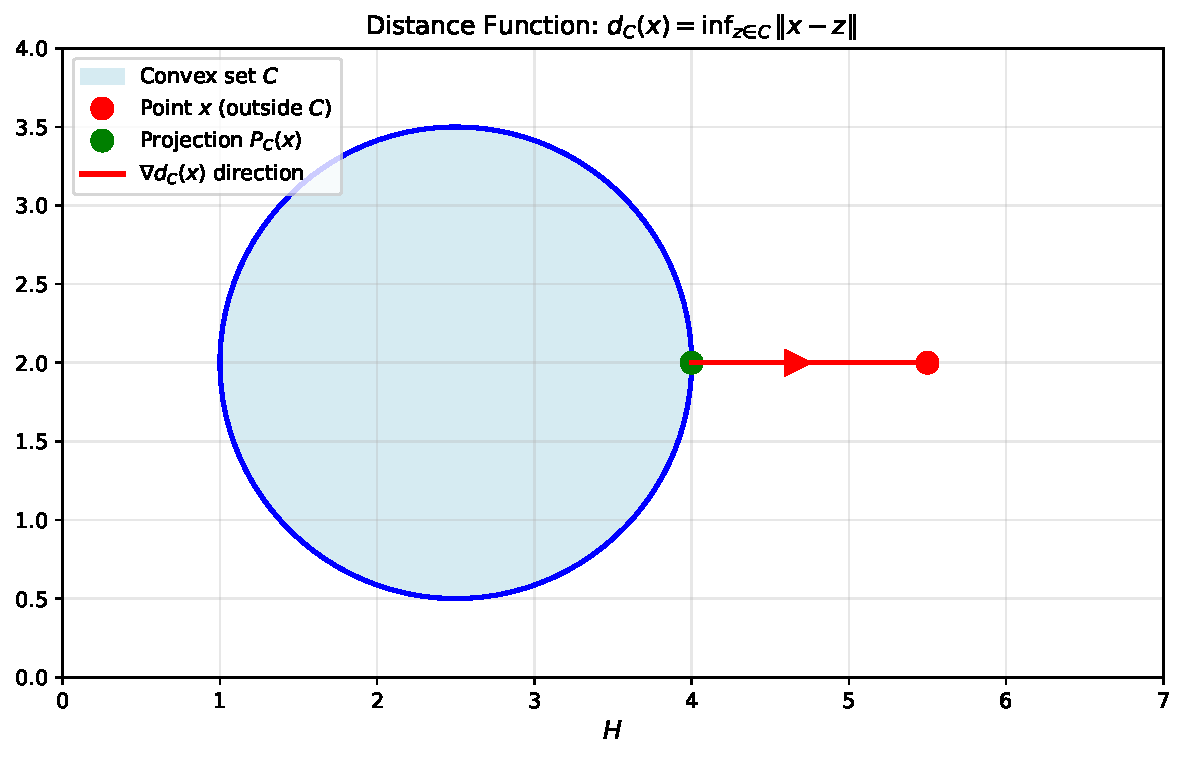
\includegraphics[width=0.65\textwidth]{fig_distance_function.pdf}

\end{frame}

\begin{frame}{Distance Function: Cases at the Boundary}

\begin{proposition}[Complete Characterization for All Points]
Let $C$ be a nonempty closed convex subset of $\mathcal{H}$ and $x \in \mathcal{H}$.

Then exactly one of the following holds:

\begin{enumerate}
  \item[(i)] Suppose that $x \in \text{int } C$. Then $d_C$ is Fréchet differentiable
            at $x$ with $\nabla d_C(x) = 0$.

  \item[(ii)] Suppose that $x \in \text{bdry } C$. Then:
    \begin{enumerate}
      \item[(a)] If $x \notin \text{spts } C$: $d_C$ is not Fréchet differentiable but
                is Gâteaux differentiable with $\nabla d_C(x) = 0$.

      \item[(b)] If $x \in \text{spts } C$: $d_C$ is not Gâteaux differentiable
                and $\partial d_C(x) = N_C x \cap B(0;1)$.
    \end{enumerate}

  \item[(iii)] Suppose that $x \notin C$. Then $d_C$ is Fréchet differentiable at $x$
              with $\nabla d_C(x) = \frac{x - P_C x}{d_C(x)}$.
\end{enumerate}
\end{proposition}

\vspace{0.2cm}

\textbf{Key Point:} The distance function has three distinct behaviors depending on
whether $x$ is interior, boundary, or exterior to $C$.

\end{frame}

% ============================================================================
% NUMERICAL EXAMPLE
% ============================================================================

\section{Numerical Examples and Applications}

\begin{frame}[fragile]{Example: Convex Quadratic Function}

\textbf{Problem:} Analyze differentiability of $f(x) = \frac{1}{2}\|x\|^2$.

\vspace{0.3cm}

\begin{lstlisting}
import numpy as np
import matplotlib.pyplot as plt

# Quadratic function: f(x) = 0.5 * ||x||^2
def f(x):
    return 0.5 * np.linalg.norm(x)**2

# Gradient (Fréchet differentiable): grad f(x) = x
def grad_f(x):
    return x

# Subdifferential at x: singleton {x}
def subdiff_f(x):
    return {np.array(x)}

# Verify Lipschitz continuity of gradient
x1 = np.array([1.0, 2.0, 3.0])
x2 = np.array([1.1, 2.1, 3.1])

grad_x1 = grad_f(x1)
grad_x2 = grad_f(x2)

# || grad f(x1) - grad f(x2) || = || x1 - x2 ||
diff_grad = np.linalg.norm(grad_x1 - grad_x2)
diff_x = np.linalg.norm(x1 - x2)

print(f"|| grad f(x1) - grad f(x2) || = {diff_grad:.6f}")
print(f"|| x1 - x2 || = {diff_x:.6f}")
print(f"Lipschitz constant beta = 1")
\end{lstlisting}

\textbf{Analysis:}
\begin{itemize}
  \item $\nabla f(x) = x$ (Fréchet differentiable everywhere)
  \item Gradient is 1-Lipschitz: $\|\nabla f(x) - \nabla f(y)\| = \|x - y\|$
  \item $(1/\beta)$-cocoercive with $\beta = 1$: firmly nonexpansive
  \item Moreau envelope: $m_\gamma(f)(x) = \frac{\gamma}{1 + \gamma}\|x\|^2$
\end{itemize}

\end{frame}

\begin{frame}[fragile]{Example: Subdifferential of Maximum}

\textbf{Problem:} Compute $\partial f(x)$ where
$f(x) = \max\{f_1(x), f_2(x)\}$ with:
$$f_1(x) = \frac{1}{2}(x+1)^2, \quad f_2(x) = \frac{1}{2}(x-1)^2$$

\vspace{0.3cm}

\begin{lstlisting}
import numpy as np

def f1(x):
    return 0.5 * (x + 1)**2

def f2(x):
    return 0.5 * (x - 1)**2

def grad_f1(x):
    return x + 1

def grad_f2(x):
    return x - 1

def subdiff_max(x):
    """Subdifferential of max{f1, f2}"""
    f1_val = f1(x)
    f2_val = f2(x)
    I_x = []

    if np.isclose(f1_val, f2_val):
        # Both active: take convex combination
        return 0.5 * (grad_f1(x) + grad_f2(x))
    elif f1_val >= f2_val:
        return grad_f1(x)  # Only f1 active
    else:
        return grad_f2(x)  # Only f2 active

# Test at intersection point x = 0
x_test = 0.0
print(f"At x = {x_test}:")
print(f"f1({x_test}) = {f1(x_test)}, f2({x_test}) = {f2(x_test)}")
print(f"Subdifferential: {subdiff_max(x_test)}")
# Both active, so subdiff = conv{1, -1} = [-1, 1]
\end{lstlisting}

\textbf{Result:}
\begin{itemize}
  \item At $x = 0$: both $f_1$ and $f_2$ are active
  \item $\partial f(0) = \text{conv}\{1, -1\} = [-1, 1]$ (interval)
  \item For $x > 0$: $f_1 > f_2$, so $\partial f(x) = \{x + 1\}$
  \item For $x < 0$: $f_2 > f_1$, so $\partial f(x) = \{x - 1\}$
\end{itemize}

\end{frame}

\begin{frame}[fragile]{Example: Distance Function to a Disk}

\textbf{Problem:} Analyze the distance function to the closed disk:
$$C = \{x \in \mathbb{R}^2 : \|x\| \leq r\}$$

\vspace{0.3cm}

\begin{lstlisting}
import numpy as np

def distance_to_disk(x, r=1.0):
    """Distance from x to closed disk of radius r"""
    x_norm = np.linalg.norm(x)
    return max(0, x_norm - r)

def grad_distance_outside(x, r=1.0):
    """Gradient of distance function when x is outside disk"""
    x_norm = np.linalg.norm(x)
    if x_norm <= r:
        return None  # Not outside
    return x / x_norm  # Unit vector from origin

# Test points
x_inside = np.array([0.2, 0.3])  # Inside disk
x_boundary = np.array([1.0, 0.0])  # On boundary
x_outside = np.array([2.0, 0.0])  # Outside disk

print(f"x_inside: d_C(x) = {distance_to_disk(x_inside):.4f}")
print(f"x_boundary: d_C(x) = {distance_to_disk(x_boundary):.4f}")
print(f"x_outside: d_C(x) = {distance_to_disk(x_outside):.4f}")

# Gradient outside
grad_outside = grad_distance_outside(x_outside)
print(f"\nAt x_outside = {x_outside}:")
print(f"grad d_C(x) = {grad_outside}")
print(f"P_C(x) = {x_outside / np.linalg.norm(x_outside)}")
# grad d_C(x) = (x - P_C(x)) / d_C(x)
\end{lstlisting}

\textbf{Results:}
\begin{itemize}
  \item Interior ($\|x\| < r$): $d_C(x) = 0$, gradient $= 0$
  \item Boundary ($\|x\| = r$): $d_C(x) = 0$, gradient $= x/\|x\|$ (outward normal)
  \item Exterior ($\|x\| > r$): $d_C(x) = \|x\| - r$, gradient $= x/\|x\|$
\end{itemize}

\end{frame}

% ============================================================================
% SUMMARY AND APPLICATIONS
% ============================================================================

\section{Summary and Applications}

\begin{frame}{Key Takeaways}

\textbf{Main Results of Chapter 18:}

\begin{enumerate}
  \item[\textbf{(i)}] \textbf{Ekeland-Lebourn:} Convex + continuous $\Rightarrow$
        dense set of Fréchet differentiability

  \item[\textbf{(ii)}] \textbf{Maximum Rule:} $\partial \max_i f_i = \text{conv} \bigcup_i \partial f_i$
        (for active indices)

  \item[\textbf{(iii)}] \textbf{Infimal Convolution:} Differentiability of $f$ at optimizer
        $\Rightarrow$ singleton subdifferential of $f \square g$

  \item[\textbf{(iv)}] \textbf{Duality:} Differentiability of $f$ $\Leftrightarrow$
        strict convexity of $f^*$

  \item[\textbf{(v)}] \textbf{Lipschitz Gradients:} Multiple equivalent characterizations
        of smooth/Lipschitz gradient property

  \item[\textbf{(vi)}] \textbf{Baillon-Haddad:} $\beta$-Lipschitz gradient $\Leftrightarrow$
        $(1/\beta)$-cocoercivity

  \item[\textbf{(vii)}] \textbf{Distance Function:} Complete characterization of differentiability
        based on position relative to set
\end{enumerate}

\end{frame}

\begin{frame}{Applications in Optimization}

\textbf{Practical Uses of Chapter 18 Results:}

\vspace{0.2cm}

\begin{itemize}
  \item \textbf{Proximal Gradient Methods:}
    \begin{itemize}
      \item Moreau envelope provides smooth approximation
      \item Lipschitz gradient characterization ensures convergence rates
    \end{itemize}

  \item \textbf{Proximal Point Algorithm:}
    \begin{itemize}
      \item Uses averaged proximal operators (Corollary 18.20)
      \item Guaranteed convergence via monotone operator theory
    \end{itemize}

  \item \textbf{Constraint Optimization:}
    \begin{itemize}
      \item Distance function characterization handles constraints
      \item Subdifferential of max handles multiple constraints
    \end{itemize}

  \item \textbf{Duality Theory:}
    \begin{itemize}
      \item Dual variables recovered from primal solutions
      \item Strict convexity of dual $\Leftrightarrow$ smoothness of primal
    \end{itemize}

  \item \textbf{Numerical Stability:}
    \begin{itemize}
      \item Smooth functions allow gradient-based methods
      \item Lipschitz constants control error bounds
    \end{itemize}
\end{itemize}

\end{frame}

\begin{frame}{Further Reading and References}

\textbf{Extensions of these results:}

\begin{itemize}
  \item \textbf{Higher-order differentiability:} Gâteaux vs. Fréchet second derivatives

  \item \textbf{Smooth approximations:} Moreau envelope generalizations, Huber loss

  \item \textbf{Variational analysis:} Coderivatives, graphical convergence

  \item \textbf{Monotone operator theory:} Connection between subdifferentials and
        monotone operators (Chapter 20-21)

  \item \textbf{Machine learning:} Lipschitz gradient bounds in neural networks,
        generalization theory

  \item \textbf{Stochastic optimization:} Large-scale versions of proximal methods
\end{itemize}

\vspace{0.3cm}

\textbf{Key Reference:}

\begin{center}
  \textit{Convex Analysis and Monotone Operator Theory in Hilbert Spaces}\\
  Heinz H. Bauschke and Patrick L. Combettes (2017)\\
  Springer-Verlag
\end{center}

\end{frame}

% ============================================================================
% APPENDIX: PROOFS AND DETAILED CALCULATIONS
% ============================================================================

\appendix

\begin{frame}[allowframebreaks]{Appendix: Descent Lemma}

\textbf{Theorem 18.15(iii): The Descent Lemma}

For a Fréchet differentiable convex function $f$ with $\beta$-Lipschitz continuous
gradient:
$$f(y) \leq f(x) + \langle y - x | \nabla f(x) \rangle + \frac{\beta}{2}\|y - x\|^2$$

\vspace{0.3cm}

\textbf{Proof:}

Let $x, y \in \mathcal{H}$. By the mean value theorem applied to the function
$\phi_z(t) = f(x + t(z - x))$:

\begin{align}
f(y) - f(x) &= \int_0^1 \langle y - x | \nabla f(x + t(y - x)) \rangle \, dt \\
&= \langle y - x | \nabla f(x) \rangle + \int_0^1 \langle y - x | \nabla f(x + t(y - x)) - \nabla f(x) \rangle \, dt
\end{align}

Using the Lipschitz property of $\nabla f$:
$$\|\nabla f(x + t(y - x)) - \nabla f(x)\| \leq \beta \cdot t\|y - x\|$$

By Cauchy-Schwarz:
$$\langle y - x | \nabla f(x + t(y - x)) - \nabla f(x) \rangle \leq \beta t \|y - x\|^2$$

Therefore:
$$\int_0^1 \langle y - x | \nabla f(x + t(y - x)) - \nabla f(x) \rangle \, dt \leq \int_0^1 \beta t \|y - x\|^2 \, dt = \frac{\beta}{2}\|y - x\|^2$$

\end{frame}

\begin{frame}{Appendix: Baillon-Haddad Proof Sketch}

\textbf{Theorem 18.17: Baillon-Haddad}

We show: $\beta$-Lipschitz gradient $\Leftrightarrow$ $(1/\beta)$-cocoercivity

\vspace{0.3cm}

\textbf{Forward direction ($\Rightarrow$):}

Assume $\|\nabla f(x) - \nabla f(y)\| \leq \beta \|x - y\|$.

By Proposition 17.35 (Fenchel-Young), for any $u \in \partial f(x)$:
$$f^*(u) \geq \langle u | x \rangle - f(x)$$

For a Fréchet differentiable $f$, we have $\partial f(x) = \{\nabla f(x)\}$, so:
$$f^*(\nabla f(x)) = \langle \nabla f(x) | x \rangle - f(x)$$

The $(1/\beta)$-cocoercivity follows from the descent lemma and properties of
the convex conjugate.

\vspace{0.3cm}

\textbf{Backward direction ($\Leftarrow$):}

Assume $(1/\beta)$-cocoercivity: $\langle x - y | \nabla f(x) - \nabla f(y) \rangle \geq \frac{1}{\beta}\|\nabla f(x) - \nabla f(y)\|^2$

This implies the Lipschitz continuity via the relationship between monotonicity
and Lipschitz properties.

\end{frame}

\end{document}
